% Chapter 2

\chapter{Method} % Write in your own chapter title
\label{Chapter:Method}
\lhead{Chapter 2. \emph{\steel}} % Write in your own chapter title to set the page header

\section{Why do we need a new modeling technique in galactic astrophysics.}
%What is missing: Massive galaxies, checks 
%How can a new model succeed where others haven't
\section{Designing to specification.}
%General format: Science problem and design solution 
%Volume/resolution - statistical
\begin{figure}[h]
    \centering
    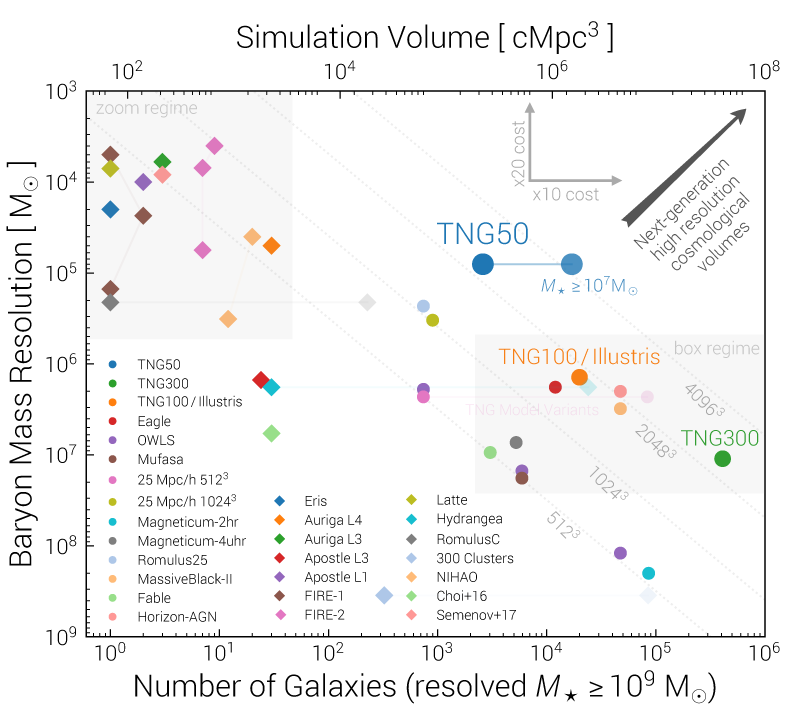
\includegraphics[width = \linewidth]{Figures/Chapter2/VolumeResolutionComparison.png}
    \caption{Image used with permission from: Illustris-TNG Project, \citet{Nelson2019FirstFeedback}}
    \label{fig:Bolshoi}
\end{figure}

%Flexibility - empirical
%Consistency - ensuring connections between high and low redshift
%Systematics - speed
\section{Modules and Methods}

\subsection{Statistical Dark matter accretion history}

%First we should explain merger trees and traditional simulation techniques.
\subsubsection{Traditional methods and merger trees}

%first n body
\begin{figure}[h]
    \centering
    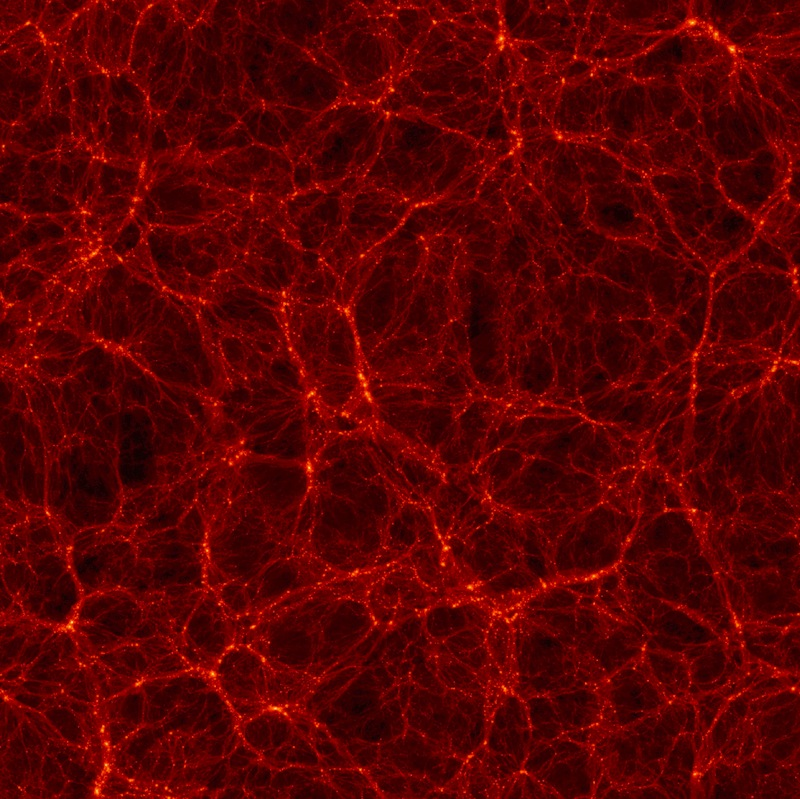
\includegraphics[width = \linewidth]{Figures/Chapter2/Bolshoi.jpg}
    \caption{Slice of the 250 Mpc$^3$ box of the Bolshoi Simulation. Brighter regions indicate a higher density of dark matter. Note the clustered bright points connected by large filaments. This structure is known as the cosmic web.
    Image credit: Bolshoi Simulation http://hipacc.ucsc.edu/Bolshoi/Images.html}
    \label{fig:Bolshoi}
\end{figure}

%then halofinders and trees (ROCKSTAR)

%then eps P08

%then hmf

%then shmf

\subsubsection{State of the art statistical method}
%then get onto what makes STEEL STEEL
\begin{figure}[h]
	\centering
	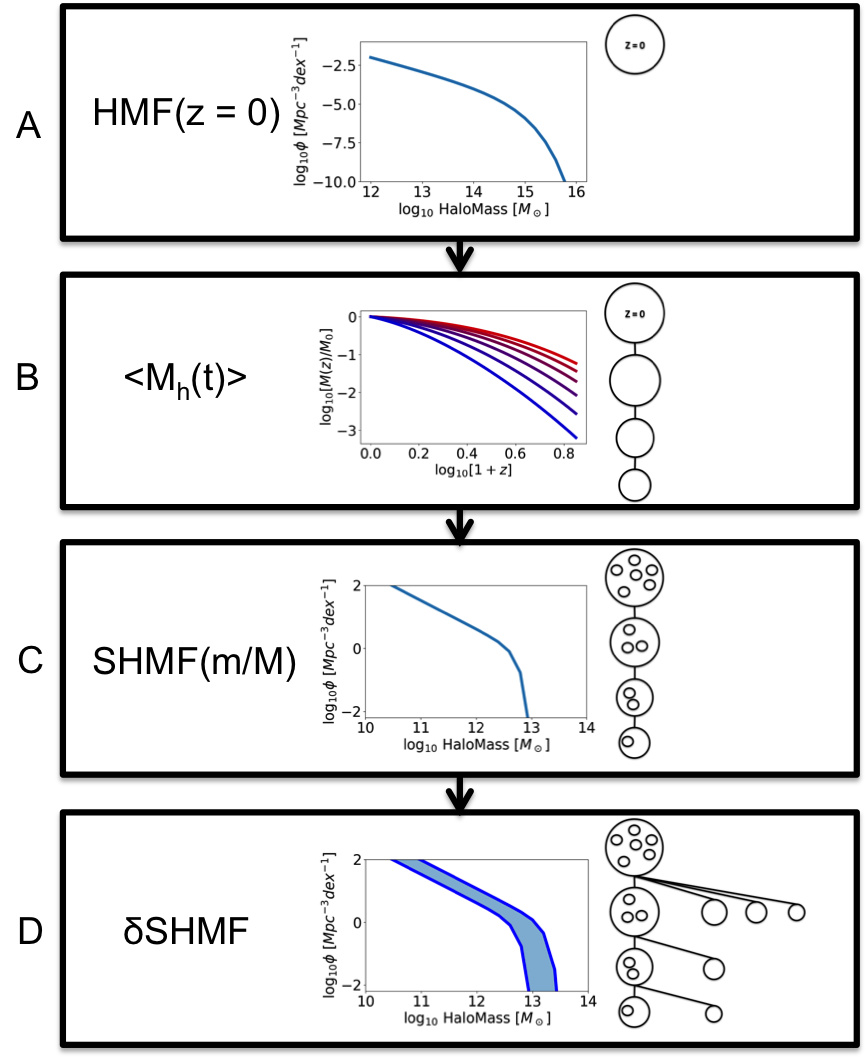
\includegraphics[width = \linewidth]{Figures/Chapter2/StatDM.png}
    \caption{I show the main steps in building the statistical dark matter accretion history for STEEL. Each panel shows a feature from a traditional merger tree and the statistical function used to replace it. A: The HMF is used to calculate the number densities of central haloes. B: Average mass growth histories are used to calculate the size of each mass bin at previous epochs. C: The (unevolved)SHMF is used to populate each central at each redshift with subhaloes. D: The average number densities of accreted subhaloes at each epoch, are calculated by taking the difference between each mass bin of the (unevolved)SHMF at consecutive redshift steps.}
	\label{fig:StatDM}
\end{figure}

\subsection{Abundance matching}
\label{C2:SubSec:AbnMtch}
\begin{figure}[h]
	\centering
	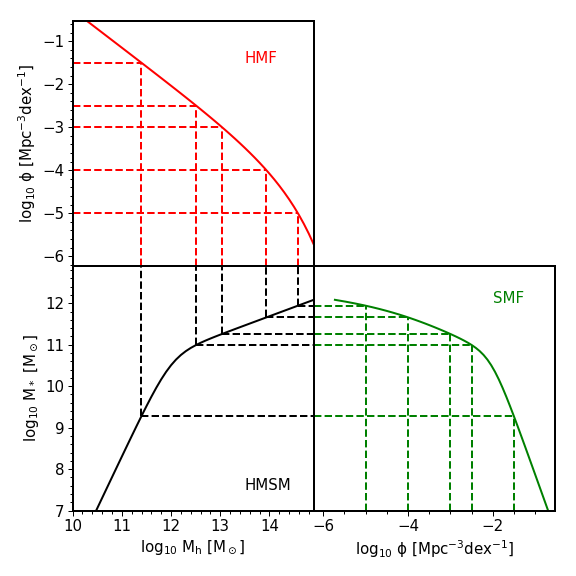
\includegraphics[width = \linewidth]{Figures/Chapter2/AbundaceMatching.png}
    \caption{A cartoon to show by matching the HMF (top left) and the SMF (bottom right) by abundance and the mapping between stellar and halo mass referred to as a SMHM relation (bottom left) is created.}
	\label{fig:Abn_Toon}
\end{figure}

\begin{figure}[h]
	\centering
	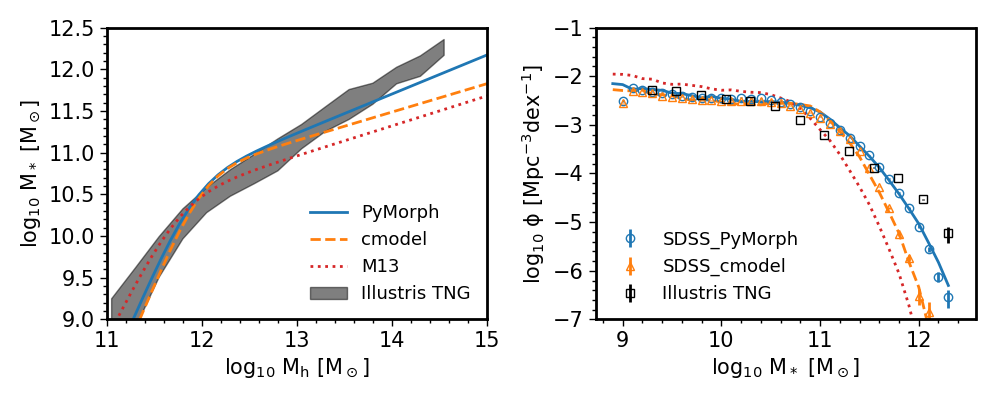
\includegraphics[width = \linewidth]{Figures/Chapter2/AbundaceMtch_Data.png}
    \caption{Left: The SMHM relation at redshift $z=0.1$. The PyMorph (blue solid line) and cmodel (orange dashed line) fits from this work are both for central haloes/galaxies, the fit from \citet{Moster2013} (M13, red dotted line) is for all haloes/galaxies. The grey band is the relation from Illustris TNG100. Right: Stellar mass functions created using the central halo mass function and the three SMHM relations compared to PyMorph (blue circles) and cmodel (orange triangles) central stellar mass functions. The black squares are the stellar mass function from Illustris TNG100.}
	\label{fig:Abn_Data}
\end{figure}

\subsection{Continuity star formation rate}
\begin{figure}[h]
	\centering
	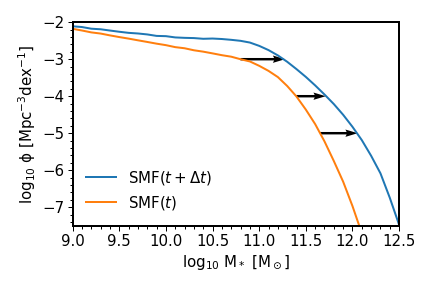
\includegraphics[width = \linewidth]{Figures/Chapter2/ContinuityEqn.png}
    \caption{The continuity approach connects at constant number density galaxy populations across cosmic time. Between two epochs `$t$' and `$t + \Delta t$' the SMF grows differently at different number density. The mass difference, $\Delta M$, indicated at three number densities by black arrows is the expected mass growth for each population.}
	\label{fig:Cont_Eqn}
\end{figure}

%Mass recycling

\begin{equation}
\label{eqn:f_ml}
f(\tau_{ml}) = 0.05 \ln \Big(\frac{\tau_{ml}}{1.4 Myr}+1\Big) ,
\end{equation}

\begin{equation}
\label{eqn:MLR}
MLR(t) = \frac{ \sum_{t' = t_{infall}}^{t} SFH(t')(f[t' - (t-\delta t)]-f[t' - t]) }{\delta t} .
\end{equation}

%Central Postprocessing 

%include a plot of using AM to convert HMGH to SMGH?
\begin{figure}[h]
	\centering
	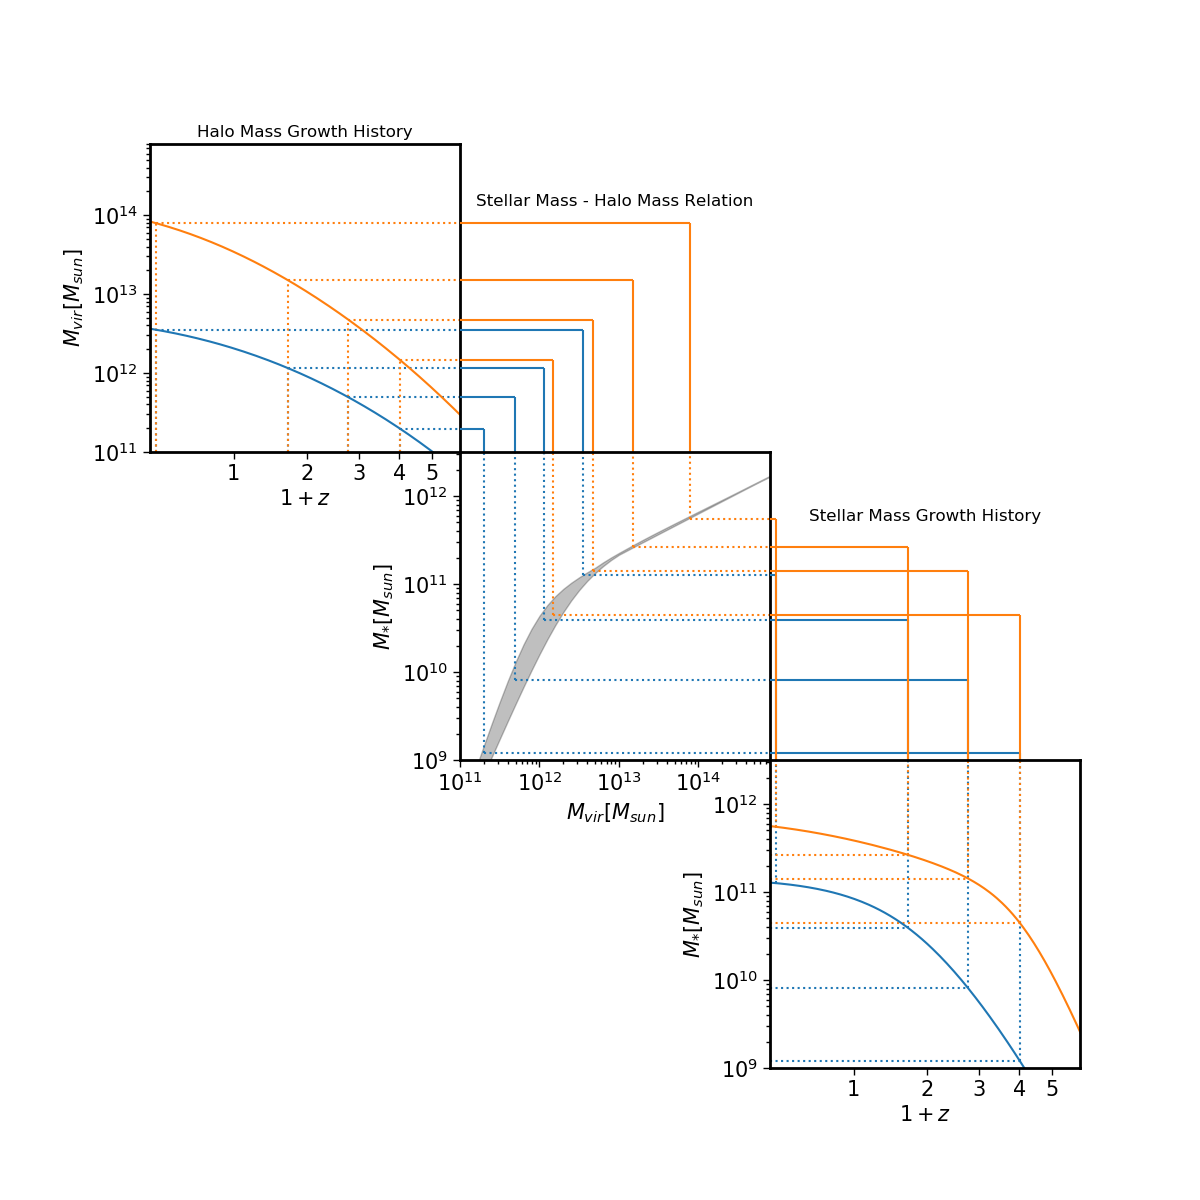
\includegraphics[width = \linewidth]{Figures/Chapter2/HMGH_to_SMGH.png}
    \caption{The Halo Mass Growth Histories (HMGH, top-left) are propagated though the redshift dependent stellar-mass-halo-mass relation (SMHM, middle) to produce corresponding Stellar Mass Growth Histories (SMGH, bottom-right). The lines illustrate matching points in redshift and the intersection with the SMHM relationship. The width of the SMHM relationship shows the extent of evolution with time, not as is common the scatter.}
	\label{fig:Cont_Eqn}
\end{figure}
